\chapter{Language Modeling: Foundations, Scale, and Efficiency}


This chapter provides a comprehensive overview of language modeling in four parts. First, we define the language modeling task and fundamental terms that are used throughout this thesis. As part of this first section, we trace through key historical milestones (e.g. n-gram models, word embeddings, and the advent of the attention mechanism and the transformer architecture). We then transition to a discussion of the current state of the art large language modeling, and key components of the modern language modeling pipeline; these include common datasets used for pretraining, common architectures, and standard evaluation benchmarks. The next section then transitions to a discussion of small langauge models, and provides an overview of recent techniques for training these types of models more efficiently. We conclude by motivating the need to explore more principled and efficient language modeling strategies, and how cognitive science can inform this effort. Key terms, concepts, and frequently referenced resources in this thesis are \thesishl{highlighted} in this chapter.

\section{How to Model Language}
\label{sec:lm-foundations}

\thesishl{Language modeling} refers to the task of assigning probabilities to sequences of words or tokens. The goal is to model the likelihood of a sequence in a language. In the case of a sequence of words, $w = w_1, w_2, \ldots, w_n$, the probability of the sequence is given by the product of the probabilities of the words occurring in the sequence:

\begin{equation}    
    P(w) = P(w_1, w_2, \ldots, w_n) = \prod_{i=1}^n P(w_i | w_1, \ldots, w_{i-1})
\label{eq:lm-joint-distribution}
\end{equation}

Training a language model is then equivalent to finding a set of parameters that maximize the likelihood of observing the training data; for this reason, language modeling is typically framed as a \thesishl{maximum likelihood estimation} problem. Configuring the parameters of a language model can be done in a number of ways, including using n-gram models, and neural language models.

\subsection{Early Approaches: N-Gram Models}
The earliest language models were based on n-gram statistics, where the probability of a word depends only on the preceding $n-1$ words. These models, described in foundational texts such as \cite{jurafsky2025speech}, are simple and effective but suffer from data sparsity and limited context. To address these issues, various smoothing techniques were developed, including Katz backoff \citep{katz2003estimation} and Kneser-Ney smoothing \citep{kneser1995improved}, with interpolated Kneser-Ney \citep{chen1999empirical} becoming the de facto standard for n-gram language modeling.

\subsection{Neural Language Models}
\label{sec:neural-language-models}

A major breakthrough came with the introduction of neural probabilistic language models by \cite{bengio2003neural}, which proposed using \thesishl{feed-forward neural networks (FFNs)} to estimate the probability of word sequences. In this formulation, the model takes as input a fixed-size context of preceding words, represented as dense vectors (see \ref{sec:word-embeddings}), and passes them through one or more fully connected layers with nonlinear activations (see activation functions in \ref{sec:optimization}). Formally, given a vectorized representation of a concatenated sequence of words $\mathbf{x} = [\mathbf{x}_1; \dots; \mathbf{x}_n]$, where each word, $w_i$, is represented as a vector $\mathbf{x}_i$, the input is processed by a feed-forward neural network as:
\begin{equation}
\mathbf{h} = \phi(W_1 \mathbf{x} + \mathbf{b}_1),
\end{equation}
\begin{equation}
\mathbf{y} = \text{softmax}(W_2 \mathbf{h} + \mathbf{b}_2),
\end{equation}
where $W_1$, $W_2$, $\mathbf{b}_1$, and $\mathbf{b}_2$ are learned parameters, $\phi$ is a non-linear function (see activation functions in \ref{sec:optimization}), softmax is defined as $\text{softmax}(x)_i = \frac{\exp(x_i)}{\sum_{j=1}^n \exp(x_j)}$ and $\mathbf{y}$ is the predicted probability distribution over the vocabulary for the next word. 

Subsequent work explored more powerful architectures, such as \thesishl{recurrent neural networks (RNNs)} \citep{mikolov2010recurrent}, which process sequences of words in a sequential, recurrent manner to capture dependencies across arbitrarily long contexts. However, training RNNs is challenging due to the vanishing and exploding gradient problems \citep{bengio1994learning}, leading to the development of gated architectures like Long Short-Term Memory (LSTM) networks \citep{hochreiter1997lstm} and Gated Recurrent Units (GRUs) \citep{cho2014gru}.

% Pretraining - Finetuning framework

% TODO


% \subsection{Neural Language Models}

% A major breakthrough came with the introduction of neural probabilistic language models by \cite{bengio2003neural}, which proposed using feed-forward neural networks to estimate the probability of word sequences. This approach introduced distributed word representations (embeddings), alleviating the data sparsity problem inherent in n-gram models. Subsequent work explored more powerful architectures, such as recurrent neural networks (RNNs) \citep{mikolov2010recurrent}, which can, in principle, capture dependencies across arbitrarily long contexts. However, training RNNs is challenging due to the vanishing and exploding gradient problems \citep{bengio1994learning}, leading to the development of gated architectures like Long Short-Term Memory (LSTM) networks \citep{hochreiter1997lstm} and Gated Recurrent Units (GRUs) \citep{cho2014gru}.
% %Large-scale empirical studies, such as \cite{jozefowicz2016exploring}, benchmarked various neural architectures and demonstrated that both model architecture and training data size significantly impact language modeling performance, as measured by perplexity.

\subsection{Word Embeddings}
\label{sec:word-embeddings}

One of the major contributions of early neural language models was the introduction and popularization of distributed, vectorized word representations, or \thesishl{word embeddings}. Neural language models were used by methods such as Skip-gram, Continuous Bag-of-Words (CBOW) \citep{mikolov2013efficient, mikolov2013distributed} and GloVe \citep{pennington2014glove} to learn dense vector representations that capture syntactic and semantic relationships between words. The output of these `embedding models' are vectorized word representations, i.e. $\mathbf{x}_i$ referenced in \ref{sec:neural-language-models}, that can be used as input to a downstream neural model that is trained to perform a particular NLP task. This two-step process of learning embeddings and then using them as input to a downstream model is a form of \thesishl{transfer learning} in NLP; learned embeddings can be used for a variety of downstream tasks, including named entity recognition~\citep{lample2016neural}, sentence classification~\citep{kim2014convolutional}, and machine translation~\citep{qi2018translation}. However, these types of `traditional' word embeddings are static, assigning the same vector to a word regardless of context.

%Some novel methods have attempted to preproces or represent the input text data in unique ways, such as \cite{kim2016character} and phoneme-level representations \cite{goriely2024babble}.

\subsubsection{Aside: Tokens vs. Words}
\label{sec:tokens-vs-words}

When discussing language modeling, we often use the terms ``words" and ``tokens" interchangeably, but they represent different concepts. While words are linguistic units with semantic meaning, \thesishl{tokens} are the atomic units that a model actually processes. Early neural language models operated directly on words, but modern approaches use tokenization algorithms to split text into \thesishl{subwords} as a preprocessing step prior to training. Tokenization algorithms usually must also themselves be trained on some set of data, to learn the optimal way to split the text into tokens. One key hyper-parameter researchers set is the \thesishl{vocabulary size}, which is the number of tokens that the model can use.

Common tokenization approaches include \thesishl{Byte Pair Encoding (BPE)} \citep{gage1994bpe, sennrich2016bpe}, which iteratively merges the most frequent character pairs; Unigram \citep{kudo2018unigram}, which starts with a large vocabulary and iteratively removes tokens to maximize the likelihood of the training data; WordPiece \citep{wu2016google}, which uses a likelihood-based merging criterion; and SentencePiece \citep{kudo2018sentencepiece}, which treats text as a sequence of Unicode characters and learns subword units directly. These subword tokenization schemes allow models to handle rare words and out-of-vocabulary terms by decomposing them into smaller, more frequent components. Throughout this thesis, we use ``tokens" to refer to these atomic processing units, whether they correspond to full words, subword pieces, or characters.

\subsection{Contextualization and Attention}
To address the limitations of static embeddings, \thesishl{attention mechanisms} were introduced, initially to solve the sequence alignment problem in machine translation \citep{bahdanau2015neural,luong2015effective}. Attention allows models to dynamically focus on the most relevant parts of the input sequence when producing each output token. More formally, given a learned \thesishl{query vector} $\mathbf{q}$ for the current word, and sets of learned \thesishl{key vectors} $[\mathbf{k}_0, \ldots, \mathbf{k}_n]$ and \thesishl{value vectors} $[\mathbf{v}_0, \ldots, \mathbf{v}_n]$ for the other words in the sequence, the attention mechanism computes a weighted sum of the values:
\begin{equation}
\text{Attention}(\mathbf{q}, K, V) = \sum_{i=1}^{n} \alpha_i \mathbf{v}_i,
\end{equation}
where the attention weights $\alpha_i$ are computed using a compatibility function, typically the \thesishl{scaled dot-product}:
\begin{equation}
\alpha_i = \frac{\exp\left(\frac{\mathbf{q} \cdot \mathbf{k}i}{\sqrt{d_k}}\right)}{\sum{j=1}^{n} \exp\left(\frac{\mathbf{q} \cdot \mathbf{k}_j}{\sqrt{d_k}}\right)},
\end{equation}
with $d_k$ denoting the dimensionality of the key vectors. 

The concept of contextual word embeddings was further advanced by models such as ELMo \citep{peters2018deep}, which extract context-sensitive representations using deep, bidirectional LSTMs. These early contextual models paved the way for the attention-based transformer architecture.

\subsection{The Transformer}
The introduction of the \thesishl{transformer} architecture by Vaswani et al.~\citep{vaswani2017attention} marked a turning point in language modeling. The transformer extended the notion of attention by introducing \thesishl{multi-head attention}, which allows the model to attend to different parts of the sequence from multiple representation subspaces simultaneously. Instead of computing a single attention function, the input is projected into multiple sets of queries, keys, and values:
\begin{equation}
\text{MultiHead}(Q, K, V) = \text{Concat}(\text{head}_1, \dots, \text{head}_h)W^O,
\end{equation}
where each head is computed as:
\begin{equation}
\text{head}_i = \text{Attention}(QW_i^Q, KW_i^K, VW_i^V).
\end{equation}
Here, $W_i^Q, W_i^K, W_i^V$ are parameter matrices for the $i$-th head, and $W^O$ is an output projection matrix that combines the outputs of the individual attention heads. This design allows each head to capture distinct types of relationships between tokens, thereby enriching the final representation.

Most importantly, the transformer model helped establish the \thesishl{pretrain-finetune} paradigm as the standard approach in modern language modeling. Rather than using static embeddings from separate models, transformer models learn contextualized representations directly from data through \thesishl{pretraining} on \thesishl{self-supervised objectives}; these are training tasks that require no human-labeled data and instead derive supervision from the structure of the text itself. These objectives, such as predicting masked tokens or next tokens in a sequence, either directly optimize the language modeling probability distribution (see \cref{eq:lm-joint-distribution}) or learn representations that indirectly capture the statistical patterns needed for language understanding. The model then adapts these learned representations to specific tasks through \thesishl{finetuning}. How to define these self-supervised objectives is the subject of the next section.


% \subsection{Contextualization and Attention}
% To address the limitations of static embeddings, attention mechanisms were introduced, initially to solve the sequence alignment problem in machine translation \citep{bahdanau2015neural,luong2015effective}. Attention allows models to dynamically focus on relevant parts of the input sequence; this was initially used to improve translation quality and enable the development of encoder-decoder architectures \citep{sutskever2014sequence}. The concept of contextual word embeddings was further advanced by models such as ELMo \citep{peters2018deep}, which extract context-sensitive representations from deep, bidirectional LSTMs.

% \subsection{The Transformer and Modern Language Models}
% The introduction of the Transformer architecture by Vaswani et al.~\citep{vaswani2017attention} marked a turning point in language modeling, The Transformer built on the earlier advances in attention mechanisms, particularly the `soft' attention mechanism of Bahdanau et al.~\citep{bahdanau2015neural}, which allowed neural machine translation models to dynamically align source and target sequences. The key contribution of the Transformer was to introduce multiple, stacked layers of attention mechanisms over the entire sequence, allowing for more efficient parallelization and the modeling of long-range dependencies.

\subsection{Transformer-based Language Models}

Building on the transformer architecture, \thesishl{BERT}~\citep{devlin2019bert} popularized the \thesishl{masked language modeling (MLM)} objective, where some percentage of input tokens are replaced with a special [MASK] token, and the model is trained to predict the original identity of these masked tokens given their context. Formally, for a sequence of tokens $T = (t_1, \ldots, t_n)$ and a set of masked positions $M \subset \{1, \ldots, n\}$, the MLM objective maximizes
\begin{equation}
    \mathcal{L}_{\text{MLM}} = \sum_{i \in M} \log P(t_i \mid t_{\setminus M}),
\end{equation}
where $t_{\setminus M}$ denotes the sequence with masked tokens replaced by [MASK]. This enables BERT to learn deep bidirectional representations, as the model can attend to both left and right context. Note that models trained to maximize the MLM objective do not directly learn a joint-distribution over the entire sequence of words as is typically assumed in language modeling (see \cref{eq:lm-joint-distribution}).

Following BERT, a number of variants improved on its design. \thesishl{RoBERTa}~\citep{liu2019roberta} removed the next sentence prediction task and scaled up training data and compute. ALBERT~\citep{lan2019albert} introduced parameter sharing and sentence order prediction to reduce model size and improve efficiency. SpanBERT~\citep{joshi2020spanbert} focused on span-level objectives for better performance on related tasks. Other architectural innovations include DistilBERT~\citep{sanh2019distilbert}, which compresses BERT via knowledge distillation, and DeBERTa~\citep{he2021deberta}, which enhances attention mechanisms through disentangled representations.

In contrast to masked language modeling, autoregressive pretraining, as used in the popular \thesishl{GPT} series~\citep{radford2018gpt1, radford2019gpt2, brown2020gpt3}, trains models to predict each token based only on its preceding context. This so-called \thesishl{autoregressive (AR)} objective maximizes the likelihood:

\begin{equation}
\mathcal{L}_{\text{AR}} = \sum_{i=1}^n \log P(t_i \mid t_1, \ldots, t_{i-1}),
\label{eq:ar-loss}
\end{equation}

enforcing a unidirectional, left-to-right dependency. Autoregressive models, in contrast to masked language models, learn a joint probability distribution over the entire sequence of words. This property makes autoregressive models `generative' models, as they can be used to sample from the learned distribution and generate text. Today, autoregressive models are the most widely used models for open-ended generation tasks.

Building on these two main paradigms, several models have explored alternative objectives and architectures. One especially influential direction is the encoder-decoder, or text-to-text, framework. T5~\citep{raffel2020t5} exemplifies this approach by casting all NLP tasks (e.g. classification, translation, question answering) as text generation problems within a unified pretraining scheme. Similarly, BART~\citep{lewis2020bart} combines a denoising autoencoder objective with a sequence-to-sequence architecture, enabling both robust understanding and fluent generation.

Other notable innovations include Transformer-XL~\citep{dai2019transformer}, which improves long-context modeling through segment-level recurrence and relative positional encodings; CTRL~\citep{keskar2019ctrl}, which allows controllable generation via conditioning on control codes; ELECTRA~\citep{clark2020electra}, which reframes pretraining as a discriminative task of replaced-token detection for improved sample efficiency; and XLNet~\citep{yang2019xlnet}, which generalizes autoregressive modeling using permutation-based objectives to capture bidirectional dependencies without masking.

Together, these advances reflect a broad exploration of architectures and training strategies in modern language modeling.

% \subsection{Alternative Architectures}
% While Transformers remain the dominant approach for language modeling, recent research has explored alternative sequence modeling approaches to address their limitations, such as quadratic complexity and long-range dependency challenges. One promising direction is state space models (SSMs). The HiPPO framework~\citep{gu2020hippo} introduced efficient memory representations for continuous-time sequences, leading to the Structured State Space Sequence (S4) model~\citep{gu2021efficiently}, which models long-range dependencies efficiently via fast convolution. Mamba~\citep{gu2023mamba} further advances SSMs with dynamic, input-dependent state transitions, achieving Transformer-level performance with linear complexity. Another notable architecture, RWKV~\citep{peng2023rwkv}, combines features of Transformers and RNNs, replacing self-attention with a time-mixed mechanism for efficient, competitive language modeling. 

% While these alternative architectures represent novel and important directions for efficient and expressive sequence modeling, in this thesis we focus primarily on Transformer-based models as the most successful and widely adopted approach for language modeling.

\subsection{Training and Optimization}
\label{sec:optimization}

The training of language models is a complex process that involves a number of different components. In this section, we will discuss the key components of the training process, including optimization algorithms, activation functions, regularization, and architectural enhancements.

\paragraph{Optimization Algorithms.} 

\thesishl{Gradient descent} is the fundamental optimization algorithm that drives neural network training. For a model with parameters $\theta$ and loss function $\mathcal{L}(\theta)$, the standard gradient descent update rule is:

\begin{equation}
    \theta_{i+1} = \theta_i - \alpha \nabla_{\theta_i} \mathcal{L}(\theta_i, D)
\end{equation}

where $\alpha$ is the \thesishl{learning rate} and $\nabla_{\theta_i} \mathcal{L}(\theta_i, D)$ is the gradient of the loss with respect to the parameters at step $i$ over a given training dataset $D$. Since the exact estimation of the gradient over the entire training dataset is computationally infeasible, modern training use an approximation of gradient descent known as stochastic gradient descent (SGD) with mini-batches \citep{robbins1951stochastic}, defined as:

\begin{equation}
    \theta_{i+1} = \theta_i - \alpha  \frac{1}{\lvert \mathcal{B}_i\rvert} \sum_{T_j \in \mathcal{B}_i} \nabla_{\theta_i} \mathcal{L}(\theta_i, T_j)
\end{equation}

where $\mathcal{B}_i \subset D$ represents the mini-batch of training examples at step $i$, and $T_j$ is the $j$-th sequence in the mini-batch. Setting the learning rate, $\alpha$, is a key hyperparameter that controls the step size of the gradient descent update, and in practice requires careful tuning throughout training.

A range of adaptive optimizers have been developed that dynamically adjust $\alpha$ over the course of optimization. These include Adagrad~\citep{duchi2011adaptive}, which adapts learning rates based on historical gradients; RMSProp \citep{tieleman2012lecture}, which normalizes updates using a moving average of squared gradients; Adam \citep{kingma2015adam}, which combines momentum with adaptive learning rates; and AdamW \citep{loshchilov2019decoupled}, which decouples weight decay from the gradient update, improving regularization behavior.

In practice, effective training of deep networks also relies on learning rate scheduling and gradient clipping. For example, the transformer architecture~\citep{vaswani2017attention} employs a learning rate schedule with an initial warm-up phase followed by inverse square root decay. Additionally, gradient clipping~\citep{pascanu2013difficulty}, which scales gradients when they exceed a threshold, is essential for preventing gradients explosion, a phenomenon that can occur when the gradients are too large and cause the model to diverge.

\paragraph{Activation Functions.} 

An \thesishl{activation function} is a mathematical operation applied to each neuron's output in a neural network, introducing nonlinearity and enabling the network to learn complex patterns. Activation functions are central to the expressiveness and trainability of neural networks. Early neural networks, as in the foundational work on backpropagation~\citep{rumelhart1986learning}, primarily used the sigmoid activation. \citet{lecun1998efficient} analyzed practical choices for activations, showing that $\tanh$ is preferable to sigmoid due to its zero-centered output, which improves optimization dynamics.

However, both sigmoid and $\tanh$ can cause gradients to shrink to zero (i.e. vanishing gradients); this occurs because the derivatives of these functions become very small when inputs are large in magnitude \citet{glorot2010understanding}. This limitation motivated the adoption of the Rectified Linear Unit (ReLU)~\citep{nair2010rectified}, defined as $\mathrm{ReLU}(x) = \max(0, x)$, which is computationally simple and alleviates vanishing gradients. ReLU became the default activation in deep learning throughout the 2010s and is still used in some lightweight transformer variants. %Variants such as Leaky ReLU~\citep{maas2013rectifier} allow a small gradient for negative inputs and helping to prevent the ``dying ReLU'' problem.

For modern language models, smoother and non-monotonic activations have proven more effective. The Gaussian Error Linear Unit (GELU)~\citep{hendrycks2016gaussian} became the default in BERT and subsequent transformers due to its empirical gains over ReLU. Swish~\citep{ramachandran2017searching}, defined as $\mathrm{Swish}(x) = x \cdot \mathrm{sigmoid}(\beta x)$, is another smooth, non-monotonic activation that performs well in deep and convolutional models. More recently, gated activations such as SwiGLU~\citep{shazeer2020glu}, which combines Swish and linear units, have outperformed ReLU and earlier GLU variants in transformer feedforward networks.

\paragraph{Regularization and Stabilization.} \thesishl{Overfitting} occurs when a model learns not only the underlying patterns in the training data but also the noise, resulting in poor generalization to new, unseen data. To address this, \thesishl{regularization} techniques such as dropout~\citep{srivastava2014dropout} are employed, which randomly deactivate units during training to encourage robustness and prevent reliance on specific features. More broadly, regularization refers to strategies designed to reduce overfitting by penalizing overly complex models or encouraging simpler, more generalizable patterns.

In addition to regularization, \thesishl{normalization} methods play a crucial role in stabilizing training and further improving generalization. Normalization involves re-scaling or shifting activations to maintain consistent distributions across layers or batches, which helps accelerate convergence and mitigate issues such as  covariate shift. Batch Normalization~\citep{ioffe2015batchnorm} normalizes activations over a mini-batch, but is less common in language models due to variable sequence lengths. Instead, \thesishl{Layer Normalization}~\citep{ba2016layernorm} is widely used in RNNs and transformers, as it normalizes across features within each data point rather than over the entire batch. RMSNorm~\citep{zhang2019rmsnorm}, a simplified variant omitting mean subtraction, is used in models like T5 \citep{raffel2020t5} and GPT-J \citep{eleutherai2021gptj}. Additionally, the placement of normalization layers has evolved: the original transformer~\citep{vaswani2017attention} used Post-Layer Normalization (layer normalization at the end of each attention layer), but this can destabilize deep models. Pre-Layer Normalization (Pre-Layer Norm)~\citep{xiong2020layer}, where normalization is applied before each sublayer, is now standard in most modern LMs for improved stability.

\paragraph{Architectural Enhancements.}
A crucial architectural component in transformer-based models is the method for encoding token position, which allows models to incorporate sequence order into otherwise permutation-invariant self-attention mechanisms. The original transformer~\citep{vaswani2017attention} introduced sinusoidal positional encodings, which are added to token embeddings and provide a fixed, non-learned way to represent absolute position. In contrast, models such as GPT~\citep{radford2018gpt1} and BERT~\citep{devlin2019bert} use learned \thesishl{fixed positional embeddings}, which offer greater flexibility but may generalize poorly to longer contexts unless specifically augmented.

To address the limitations of absolute position encodings, \citet{shaw2018self} proposed \thesishl{relative position representations}, allowing the model to encode the distance between tokens directly in the attention mechanism. This approach is particularly important for enabling models to generalize to longer contexts and to be less dependent on a fixed sequence length. Further innovations include linear attention biases (ALiBi)~\citep{press2021train}, which add a simple, non-learned bias to the attention scores based on token distance. Another widely adopted method is the Rotary Position Embedding (RoPE)~\citep{su2024rope}, which applies rotary transformations to the key and query vectors in the attention mechanism. RoPE has become popular in many large models, such as LLaMA, due to its ability to extrapolate to longer sequence lengths.

Beyond positional encoding, several other architectural enhancements have become standard in modern transformers. \thesishl{Residual connections}~\citep{he2016deep}, originally introduced in ResNets to address vanishing gradients, are essential for enabling the training of deep transformer models by facilitating gradient flow. More recent innovations include \thesishl{Grouped Query Attention} (GQA)~\citep{ainslie2023gqa}, which reduces memory and compute requirements by grouping multiple attention heads to share key and value projections; GQA is now adopted in models such as Gemini \citep{deepmind2023gemini}, PaLM \citep{chowdhery2023palm}, and LLaMA \citep{touvron2023llama}. Additionally, parameter efficiency has been improved through \thesishl{weight tying}~\citep{press2017using}, where the input and output embedding matrices are shared, reducing the number of parameters without sacrificing performance.

\subsection{Scaling and Architecture Search}
While recent research has shown that scaling model and dataset size leads to predictable improvements in performance~\citep{kaplan2020scaling, henighan2020scaling}, designing neural network architectures in a robust and rigorous way remains a significant challenge. Much of architecture design is still guided by empirical intuition and trial-and-error, rather than first principles. For example, \citet{levine2020depth} offer a structured perspective on the trade-offs between scaling depth and width in Transformers, proposing guidelines for balancing these factors under a fixed compute budget. The scaling laws established by \citet{kaplan2020scaling} demonstrate that both wider and deeper models can improve performance if scaled appropriately, but do not prescribe how to select specific architectural configurations for a given task or resource constraint.

To address the difficulty of manual architecture design, neural architecture search (NAS) methods have been developed to automate this process. Early work by \citet{zoph2017neural} introduced the use of reinforcement learning to train a controller network that proposes architectures that uses the accuracy of candidate models as a reward signal. More recent approaches have applied NAS specifically to transformer models: AutoFormer~\citep{chen2021autoformer} efficiently searches over large design spaces (such as number of heads, depth, and MLP size) using weight-sharing, while NAS-BERT~\citep{xu2021nasbert} tailors BERT-like architectures for specific NLP tasks, reducing model size while maintaining performance through task-conditioned optimization.

Despite these advances, finding good architectures remains challenging and is difficult to do in a robust and scientific way.

\section{Large Language Models}

The advent of large language models (LLMs) has represented a turning point in natural language processing. Unlike earlier models, which were limited by data and compute, LLMs are trained on massive corpora (on the order trillions of tokens) and contain billions or even trillions of parameters. This scale enables them to perform a wide range of tasks, including question answering, summarization, translation, and code generation, often with little or no task-specific training. It is important to note, however, that the definition of ``large'' in large language models is a moving target: as models and hardware have advanced, what was once considered large has quickly become standard or even small by contemporary benchmarks.

The rapid progress in large language models has been marked by influential systems, each pushing the boundaries of scale, and capability. GPT-3~\citep{brown2020gpt3} was one of the first to establish the transformative potential of large transformer-based models, enabling a model to peform well on a range of tasks with little to no task-specific training. Since then, models like Anthropic's Claude~\citep{anthropic2024claude3,anthropic2024claude35,anthropic2025claude37}, Google's Gemini~\citep{deepmind2023gemini}, Baidu's ERNIE 4.0~\citep{baidu2023ernie4}, and Alibaba's Qwen~\citep{alibaba2023qwen} have demonstrate advancements in multimodality, multilingual support, and long-context reasoning to solve tasks in a range of domains, such as coding and math. In addition to closed propriety models, open-source language models (often published by private companies) have also significantly advanced our understanding of large language models. These include DeepSeek LLM~\citep{deepseek2024llm}, Mistral 7B~\citep{jiang2023mistral}, PaLM~\citep{chowdhery2023palm}, OPT~\citep{zhang2022opt}, and BLOOM~\citep{le2023bloom}. 

The following section explores some of the critical aspects of large language models including their pre-training datasets, large-scale evaluation benchmarks, and properties.

\subsection{Datasets for Large Language Model Pretraining}
The performance of large language models (LLMs) is strongly influenced by the scale, diversity, and quality of their pretraining datasets. Over the past several years, a number of large-scale corpora have been developed to support open and reproducible LLM research. Table~\ref{tab:llm-datasets} summarizes some of the most widely used datasets.

\begin{table}[ht!]
    \centering
    \renewcommand{\arraystretch}{1.3}
    \setlength{\tabcolsep}{5pt}
    \begin{tabular}{p{2.8cm} c | c c c c c c}
    \toprule
    % \rowcolor{thesisblue!20}
    \textbf{Dataset} & \textbf{\# Tokens} & \textbf{Web} & \textbf{Books} & \textbf{Code} & \textbf{Academic} & \textbf{Forums} & \textbf{Wiki} \\
    \midrule
    BooksCorpus  & ~0.8B   &            & \cmark  &         &          &            &             \\
    OpenWebText  & ~8B     & \cmark &             &         &          & \cmark &             \\
    \thesishl{The Pile}     & ~250B   & \cmark & \cmark  & \cmark & \cmark & \cmark &             \\
    C4           & ~365B   & \cmark &             &         &          &            &             \\
    RefinedWeb   & ~600B   & \cmark &             &         &          &            &             \\
    RedPajama    & ~1,200B   & \cmark & \cmark  & \cmark & \cmark & \cmark & \cmark \\
    \thesishl{DOLMa}        & ~3,000B     & \cmark & \cmark  & \cmark & \cmark & \cmark & \cmark \\
    FineWeb      & ~15,000B    & \cmark & \cmark  &         &          &            & \cmark \\
    \bottomrule
    \end{tabular}
    \caption{Major LLM pretraining datasets with approximate token counts (in billions, B) and data type coverage.}
    \label{tab:llm-datasets}
\end{table}

These datasets are constructed from a variety of sources, including web pages (Common Crawl), books, academic papers, code repositories, and community forums. Notably, OpenWebText and BooksCorpus were foundational for early models like GPT-2 \citep{radford2019gpt2} and BERT \citep{devlin2019bert}, while The Pile and C4 introduced greater diversity and scale and were used to train models like GPT-j \citep{eleutherai2021gptj}. More recent efforts such as RedPajama, RefinedWeb, FineWeb, and DOLMa focus on quality filtering, and massive scale, and are used to train the newest set of LLMs like OLMo \citep{groeneveld2024olmo}.

\subsection{Evaluation Benchmarks for Large Language Models}
The advancement of large language models (LLMs) has also been driven by the development of rigorous evaluation benchmarks. These benchmarks assess a model's ability to understand, reason, and generate language across a wide range of tasks. Below, we summarize some of the most influential benchmarks used to evaluate LLMs.
\paragraph{GLUE and SuperGLUE.} The General Language Understanding Evaluation (GLUE) benchmark \citep{wang2018glue} popularized the paradigm of transfer learning and fine-tuning in NLP. It consists of nine tasks, including natural language inference (MNLI, RTE) \citep{williams2018mnli,dagan2006rte}, paraphrase detection (MRPC) \citep{dolan2005mrpc}, sentiment analysis (SST-2) \citep{socher2013sst}, linguistic acceptability (CoLA) \citep{warstadt2019cola} and semantic similarity (STS-B) \citep{cer2017stsb}. BERT's breakthrough performance on GLUE established it as a standard benchmark; since BERT, models such as Roberta \citep{liu2019roberta} and T5 \citep{raffel2020t5}, have achieved near-perfect performance on GLUE, rendering the benchmark trivial for modern LLMs. \thesishl{SuperGLUE} \citep{wang2019superglue} was introduced as a more challenging successor, featuring tasks that require multi-sentence reasoning, commonsense inference, and coreference resolution \citep{zhang2018record,pilehvar2019wic,khashabi2018multirc,roemmele2011copa}. Progress on these benchmarks has closely tracked advances in LLM capabilities.

\paragraph{MMLU.} The Massive Multitask Language Understanding (MMLU) \citep{hendrycks2021mmlu} benchmark evaluates models on 57 diverse tasks spanning STEM, humanities, law, and more, using multiple-choice questions. MMLU emphasizes zero-shot and few-shot generalization, and is now a standard for evaluating the broad knowledge and reasoning abilities of frontier LLMs such as GPT-3 \citep{brown2020gpt3}, GPT-4 \citep{openai2023gpt4}, Claude \citep{anthropic2024claude3}, and LLaMA \citep{touvron2023llama}.

\paragraph{ARC.} The AI2 Reasoning Challenge (ARC) \citep{clark2018arc} tests scientific and commonsense reasoning using grade-school multiple-choice questions. The challenge set is specifically designed to be unsolvable by information retrieval alone, requiring genuine reasoning and world knowledge.

\paragraph{BIG-Bench and BIG-Bench Hard.} The Beyond the Imitation Game Benchmark (BIG-Bench) \citep{suzgun2023bigbenchhard} is a large-scale suite of over 200 tasks covering math, code, ethics, linguistics, and more, designed to probe

\paragraph{HellaSwag.} \thesishl{HellaSwag}~\citep{zellers2019hellaswag} is a commonsense inference benchmark that evaluates a model's ability to complete sentences in a grounded and contextually appropriate manner. Each example presents a context followed by four possible sentence endings, and the model must select the most plausible continuation. HellaSwag is specifically designed to be challenging for language models by minimizing the effectiveness of superficial statistical cues, thereby requiring genuine understanding of everyday scenarios and commonsense reasoning. This benchmark is widely used to assess whether models can move beyond surface-level pattern matching to deeper contextual comprehension.

\paragraph{Intrinsic Evaluation: Perplexity and Linguistic Probes.} 
\thesishl{Perplexity} \citep{jelinek1977perplexity} is a standard intrinsic metric for evaluating language models. It measures how well a model predicts a sequence of text, defined as the exponentiated average negative log-likelihood of the true tokens under the model; in practice, this can be computed by exponentiating the AR loss, see \cref{eq:ar-loss}. Lower perplexity indicates better predictive performance, reflecting how closely a model's probability distribution aligns with the actual data. While widely used, perplexity does not fully capture a model's understanding of linguistic structure, coherence, or factuality.

Recent work has emphasized the importance of broader evaluation frameworks. For instance, \thesishl{Paloma} \citep{magnusson2024paloma} assesses how well language models match the statistical properties of natural text, essentially functioning as a large-scale perplexity-inspired probe across multiple domains. Similarly, linguistic benchmarks such as \thesishl{BLiMP} and MSGS \citep{warstadt2020blimp, warstadt2020msgs} use controlled minimal pairs to test for grammaticality, implicitly relying on the assumption that a well-calibrated language model will assign lower perplexity to grammatical over ungrammatical constructions.

% Together, these evaluations offer complementary views of model performance—from raw predictive accuracy to nuanced linguistic competence—and highlight the ongoing need for diverse and challenging benchmarks as models scale in capability.

% \subsection{Properties of Large Language Models}

% In addition to their evaluation performance, large language models (LLMs) exhibit a range of remarkable properties that set them apart from earlier generations of language models. As these models have grown in scale and sophistication, researchers have observed the emergence of new abilities, improved generalization, and the development of empirical scaling laws that guide model design. %In addition, a suite of post-training methods has been developed to further enhance LLM capabilities and align them more closely with human preferences.

% \paragraph{Emergent Abilities}

% A striking phenomenon in LLMs is the appearance of emergent abilities; these are capabilities that seemingly arise unpredictably as model size increases. For example, certain tasks such as arithmetic reasoning and multi-step problem-solving are only performed successfully by models beyond a specific scale \citep{{wei2022emergent}}. Some studies reveal that performance on particular tasks follows U-shaped or inverted-U scaling curves, allowing for the prediction of emergence thresholds and future performance \citep{wu2024u}. However, this unpredictability has been challenged, with some recent work suggesting that emergent abilities may be artifacts of how performance is measured, and that with appropriate evaluation, their appearance can be anticipated \citep{schaeffer2023mirage, wei2022chain}.


% \paragraph{Generalization}

% Closely related to emergence is the property of generalization. LLMs are able to perform well on unseen data, often surpassing expectations for overparameterized models \citep{belkin2019reconciling}. Research has shown that increasing model capacity beyond the point of interpolation can actually improve test performance, depending on the task, in a phenomenon known as deep double descent. For instance, many few-shot prompting abilities only emerge in models with 100-500B parameters whose training processes surpasses 1E+23 flops of computation. \citet{yilmaz2022regularization} provide a theoretical exploration of why double descent occurs that relate to interpolation threshold, noise, and regularization; these insights provide a guide for how and when overparameterized models avoid overfitting. 

% \paragraph{Scaling Laws}

% The development and scaling of LLMs have been guided by empirical scaling laws, which describe how model performance depends on factors such as model size, dataset size, and compute. \citet{kaplan2020scaling} establish a power-law relationship between these factors, recommending making models bigger while keeping the training dataset size relatively fixed. \citet{henighan2020scaling} extend these laws to a multimodal setting, showing that larger models continue improving even on out-of-distribution data. \citet{hoffman2022chinchilla} introduce the Chinchilla model, finding that models trained with more data for longer, but with fewer parameters, perform better for the same amount of compute, suggesting that data size should scale more aggressively than model size to be compute-optimal. \citet{hernandez2021scaling} explore how scaling affects transfer performance to downstream tasks, finding that larger models require less fine-tuning data, and downstream task performance also follows predictable scaling curves.

% \subsection{Post-Training Methods for Large Language Models}

% Beyond pretraining, recent advances in LLMs have been driven by sophisticated post-training methods that enhance factuality, alignment, and task performance. One prominent direction is retrieval-augmented generation (RAG), which adds non-parametric memory to language models~\citep{lewis2020retrieval}. This approach enables LLMs to access up-to-date and domain-specific information beyond their training data, achieving state-of-the-art results on knowledge-intensive tasks. Some models, such as Command R+~\citep{cohere2024commandrplus}, are fine-tuned specifically for retrieval-augmented workflows and to improve their factual accuracy.

% Another major area of post-training is alignment with human preferences and instructions. Reinforcement learning from human feedback (RLHF)~\citep{christiano2017deep, ouyang2022training} with Proximal Policy Optimization (PPO)~\citep{schulman2017proximal} has become a standard method to fine-tune models using reward signals from human preference data. Direct Preference Optimization (DPO)~\citep{rafailov2023direct} is an alternative approach that directly optimizes model parameters from preference data, bypassing the need for a separate reinforcement learning loop. This method is used in recent open-source models such as Zephyr~\citep{huggingface2023zephyr}, which are chat-tuned for high-quality conversational performance. Instruction finetuning is another effective post-training strategy. Models like InstructGPT~\citep{ouyang2022training} and FLAN~\citep{wei2021flan} are further trained on instruction datasets, often with human feedback, that greatly improving their ability to follow instructions, and generate helpful outputs. Within instruction finetuning, including chain-of-thought reasoning in the finetuning data has been shown to further boost performance on complex tasks \citep{wei2022chain}.

% Collectively, these post-training methods are critical for aligning LLMs with human values, improving factuality, and enabling robust performance across a wide range of real-world applications.

\section{Small Language Models}

The landscape of language modeling has rapidly expanded beyond massive models like GPT-3 and GPT-4, giving rise to a vibrant ecosystem of smaller language model frameworks. Several open-source projects, such as the OPT language model family~\citep{zhang2022opt}, \thesishl{Pythia} \citep{biderman2023pythia} and OLMo \citep{groeneveld2024olmo}, have played a key role in democratizing access to large-scale language modeling by releasing models of varying sizes (including sub-1 biliion parameter models) and making their implementations widely available. Other initiatives, such as LaMini-LM~\citep{wu2024lamini} and TinyLlama~\citep{zhang2024tinyllama}, have focused on developing tiny-scale, instruction-tuned models similar to ChatGPT that are capable of following instructions and solving language understanding tasks.

In parallel, the demand for on-device deployment and cost-effective inference has spurred the development of numerous small language model suites. Frameworks such as MobileLLM~\citep{liu2024mobilellm} and Microsoft's Phi-3~\citep{abdin2024phi} are specifically optimized for mobile and resource-constrained environments, addressing challenges related to latency, memory, and on-device efficiency. Other projects, including Apple's OpenELM~\citep{mehta2024openelm} and MobiLlama~\citep{thawakar2024mobillama}, focus on minimizing battery consumption through energy-efficient model architectures.

Together, these frameworks reflect the demand for practical small models that can be deployed on-device, and are more accessible to the general public. In the following section, we will examine a broad set of existing strategies to make small language models more efficient to train and deploy.

\subsection{Hyper-Parameter Selection}

Recent work has shown that simply carefully tuning hyper-parameter selection can dramatically improve the efficiency and performance of small language models, even under tight computational constraints. Approaches such as targeted architectural choices~\citep{hillier2024super}, optimized training schedules and mixed-precision techniques~\citep{izsak2021train}, and aggressive learning rate strategies~\citep{geiping2023cramming} enable strong results on standard benchmarks using limited resources.

\subsection{Software Packages}

A number of specialized software frameworks have been developed to enable efficient training of large language models on modern hardware. Megatron-LM~\citep{narayanan2021megatron} and \thesishl{DeepSpeed}~\citep{rasley2020deepspeed} introduce advanced parallelism strategies and memory optimizations, such as tensor and pipeline model parallelism, ZeRO redundancy optimizer \citep{rajbhandari2020zero}, and 3D parallelism, allowing models to be trained efficiently across GPU clusters. These tools target hardware efficiency, making language modeling pre-training feasible with limited resources.

\subsection{Knowledge Distillation}

Knowledge distillation is a central technique for training small language models, particularly in data-limited settings. Here, a compact `student' model learns to replicate the behavior of a larger `teacher' to improve the training efficiency and performance of the smaller model.
Recent studies show that distillation can be highly effective even when both teacher and student are small. For example, \citet{timiryasov2023baby} and \citet{tastet2024babyllama2} demonstrate that distilled models can outperform their teachers and baselines on the BabyLM benchmark \citep{warstadt2023babylm1, conll2024babylm2}. \citet{yam2024tinyminds} further show that careful distillation design can yield gains even with compact models, improving on strong baselines like LTG-BERT~\citep{samuel2023ltgbert}.
Distillation is also used in widely adopted models such as DistilBERT~\citep{sanh2019distilbert}, which achieves a more efficient version of BERT with minimal accuracy loss, and Deepseek-r1~\citep{guo2025deepseekr1} which uses distillation from a larger Qwen model~\citep{alibaba2023qwen} to improve reasoning abilities in the student.

\subsection{Pruning}

Unlike knowledge distillation, which transfers knowledge from a larger teacher to a smaller student model, pruning directly reduces model size by removing unnecessary weights or connections from a trained network. This approach aims to create sparse, efficient models without requiring a separate teacher.
Early work such as Optimal Brain Damage~\citep{lecun1990optimal} and Optimal Brain Surgeon~\citep{hassibi1993optimal} introduced principled pruning based on second-order derivatives of the loss, identifying and removing weights with minimal impact on performance. Later, magnitude-based pruning~\citep{han2015learning} offered a scalable alternative by eliminating low-magnitude weights, followed by retraining to recover accuracy. This method was extended in Deep Compression~\citep{han2016deep}, which combines pruning, and quantization to dramatically reduce model size for deployment on devices like smartphones.
The \thesishl{Lottery Ticket Hypothesis}~\citep{frankle2019lottery} further showed that large, dense networks contain sparse subnetworks (“winning tickets”) that can be trained to match the original model's accuracy, suggesting that much of a model's capacity is redundant. More recently, efficient single-shot pruning methods such as Wanda~\citep{sun2024simple} have been proposed, using weight magnitude and input activation norms to identify important weights without iterative retraining.
Pruning thus provides a complementary path to model efficiency, by enabling substantial reductions in size and compute while maintaining strong performance.

\subsection{Architecture}

Modifications to the architecture of language models remains one of the most common approaches for improving the efficiency of language models. In this section, we outline key approaches that have been proposed to reduce parameter count, memory usage, and computational cost.

\paragraph{Weight Decomposition}
A number of recent models exemplify these architectural innovations. LTG-BERT~\citep{samuel2023ltgbert}, for instance, uses `disentangled attention' to separately encode content and positional information within the attention mechanism, thereby enhancing representational power without increasing model size. MobiLlama~\citep{thawakar2024mobillama} is designed for lightweight deployment and employs grouped query attention and shares weights between feed-forward layers to reduce redundancy and memory footprint. Similarly, MobileLLM~\citep{liu2024mobilellm} targets on-device applications by reducing model latency through deep, thin architectures that utilize embedding sharing and block-wise grouped query attention for efficient inference. ALBERT~\citep{lan2019albert} further demonstrates the benefits of parameter sharing by tying the weights of both feed-forward and attention layers across the network, significantly reducing model size while maintaining strong performance.

\paragraph{Mixture-of-Experts and Conditional Computation}
Another major direction for architectural efficiency is the use of Mixture-of-Experts (MoE) and conditional computation, where only a subset of model parameters are activated for each input. The foundational idea was introduced by \citet{jacobs1991adaptive}, who proposed a gating mechanism to dynamically route information to different expert subnetworks, allowing the model to specialize and improve efficiency. Building on this, \citet{shazeer2017outrageously} demonstrated the effectiveness of sparsely-gated MoE layers in large-scale neural networks, applying conditional computation to language modeling and machine translation, initially with LSTM-based architectures. The approach was further advanced by Switch Transformers~\citep{fedus2021switch}, which implemented MoE within the transformer framework for the first time, achieving up to a 7x increase in pre-training speed on T5-based models by activating only a subset of experts per input. More recently, Mixtral of Experts~\citep{jiang2024mixtral} introduced a sparse MoE architecture based on Mistral 7B, where each feedforward block selects from eight distinct expert groups, and a router network chooses two experts per token at each layer. %GShard~\citep{lepikhin2020gshard} further contributed by introducing automatic sharding techniques for MoE architectures, facilitating the training of giant models across distributed hardware. %The Deepseek-v3 model~\citep{deepseek2024v3} combines MoE with multi-head latent attention, exemplifying the latest advances in leveraging expert specialization and conditional computation for both scalability and efficiency in modern language models.

\paragraph{Sparse and Efficient Attention Mechanisms}
A central challenge in scaling language models is the quadratic computational and memory cost of standard self-attention, which motivates a wide range of approaches for making attention more efficient and scalable. Early work such as \citet{luong2015effective} introduced local attention for neural machine translation, restricting the attention mechanism to a fixed window around each token and thereby reducing computation by focusing only on relevant parts of the surrounding input. Building on this, a series of sparse attention mechanisms have been proposed to further improve efficiency for long sequences. The Sparse Transformer~\citep{child2019generating} utilizes a combination of strided and fixed attention patterns across layers, reducing complexity from $O(n^2)$ to $O(n\sqrt{n})$. The Routing Transformer~\citep{roy2020efficient} employs content-based sparse attention by dynamically clustering tokens using online k-means, achieving $O(n^{1.5})$. complexity. Longformer~\citep{beltagy2020longformer} and BigBird~\citep{zaheer2020big} combine local windowed attention with global and random attention patterns, enabling linear scaling with sequence length while maintaining strong empirical and theoretical performance. Reformer~\citep{kitaev2020reformer} introduces locality-sensitive hashing to group similar tokens into buckets, performing attention only within buckets and reducing complexity to $O(n\log(n))$. Linformer~\citep{wang2020linformer} projects key and value matrices to a lower dimension, leveraging the low-rank property of attention matrices to achieve linear complexity. LongNet~\citep{ding2023longnet} proposes a hierarchical, dilated attention pattern that, when combined with stacked layers, allows models to attend to a wide range of tokens efficiently, scaling to extremely long sequences. More recent innovations include attention sinks~\citep{xiao2023attentionsink}, which introduce special tokens that accumulate attention and serve as memory `anchors'. 

In addition to algorithmic sparsity, hardware-aware optimizations have also played a crucial role. \thesishl{FlashAttention}~\citep{dao2022flashattention} and its successor FlashAttention-2~\citep{dao2023flashattention2} achieve dramatic speed and memory improvements by tiling the attention computation to fit on-chip memory, minimizing slow memory accesses and fusing operations into a single GPU kernel. These methods compute exact softmax attention (unlike many sparse or approximate methods), enabling models to process much long sequences without sacrificing accuracy or requiring architectural changes. FlashAttention-2 further improves efficiency by supporting variable-length sequences and mixed precision,  Collectively, these advances in sparse and efficient attention mechanisms have been instrumental in enabling the training and deployment of large language models on long-context tasks and resource-constrained hardware.

\paragraph{Adapters and Parameter-Efficient Fine-Tuning}

For fine-tuning large pre-trained models on downstream tasks, adapters and parameter-efficient fine-tuning (PEFT) methods have become essential. Instead of updating all model parameters, these approaches introduce small trainable modules or selectively update a subset of parameters, greatly reducing computational and memory costs. LoRA~\citep{hu2021lora} is a popular PEFT method that injects low-rank trainable matrices into attention and feed-forward layers of a trained model; finetuning only requires adapting the minimal parameters added by LoRA. ReLoRA~\citep{lialin2023relora} extends this by using low-rank updates for faster, more memory-efficient training. Other common PEFT strategies include BitFit~\citep{benzaken2022bitfit}, which updates only bias terms, and (IA)$^3$~\citep{liu2022few}, which scales large, fixed activations with small learned vectors. Tools like HuggingFace's PEFT library have made these techniques widely accessible, enabling rapid and cost-effective adaptation of large models to new tasks.

%Early work in vision~\citep{rebuffi2017adapters} added residual adapter modules, while in NLP, \citet{houlsby2019parameter} proposed lightweight down- and up-projection layers within Transformers. L


\subsection{Quantization}
Quantization reduces the memory and compute demands of models by representing weights and activations with low-precision values. BitNet~\citep{wang2023bitnet} achieves extreme efficiency by binarizing weights to a single bit and scaling activations with an absmax function, while keeping gradients in full precision. Activation-Aware Weight Quantization~\citep{lin2023awq} preserves accuracy by expanding the range of the most important weights, minimizing distortion from low-bit quantization. QLoRA~\citep{dettmers2023qlora} is a quantized version of LoRA that enables efficient fine-tuning of 4-bit quantized models, making it possible to adapt large models like LLaMA-65B on a single GPU. Underpinning many quantization methods is the Straight-Through Estimator (STE)~\citep{bengio2013estimating}, which allows gradients to flow through non-differentiable quantization operations. Together, these advances make it feasible to compress and deploy large models in resource-limited settings.

\subsection{Data Calibration}
Recent research challenges the long-standing assumption that massive datasets are necessary for effective language modeling. A growing body of work shows that carefully calibrated training data can enable small models to perform surprisingly well, especially when the input is tailored to the specific competencies we want the model to acquire.

The \thesishl{BabyLM Challenge}~\citep{warstadt2023babylm1, conll2024babylm2} (hosted at the CoNNL workshop) exemplifies this shift in perspective. The goal of the challenge is to test the limits of language model training under data-constrained settings that loosely mirror how infants are exposed to language. In particular, the challenge requires researchers to train small language models on only a very limited dataset of `cognitively-plausible' data (10 million words). The dataset provided by the organizers is carefully curated to reflect the kinds of input that infants and young children receive during early language acquisition. The dataset includes:

\begin{itemize}
    \item Child-directed speech, drawn from corpora like CHILDES~\citep{macwhinney2000childes}, to reflect simplified, interactive language used by caregivers.
    \item Children's literature and narrative text, offering simple syntactic structures and familiar vocabulary.
    \item Dialogues and story transcripts, capturing conversational patterns common in early learning environments.
    \item Simple English Wikipedia, which maintains informative content while reducing linguistic complexity.
\end{itemize}

This aim is for the data composition to somewhat reflect the developmental trajectory of human learners (from simple utterances spoken by care-givers to children stories to basic Wikipedia articles). By emulating this, the BabyLM Challenge offers a principled alternative to large-scale pretraining regimes.

Outside of the BabyLM Challenge, research projects have demonstrated that training on developmentally-plausible data can be beneficial to more efficiently training small language models. For instance, TinyStories~\citep{eldan2023tinystories} demonstrates that small models can learn coherent text generation from just 1.3 million synthetic stories written in a limited vocabulary. Similarly, BabyBERTa~\citep{huebner2021babyberta}, trained on only 5 million words of child-directed speech, achieves strong grammatical competence with a tiny model footprint. These results emphasize that the structure, and content of training data can be as important as the amount of data. 

The BabyLM Challenge not only consolidates these ideas, but also serves as a testbed for cognitively-inspired training paradigms, including curriculum learning.

\section{Human-Centered Language Modeling}

\begin{figure}[ht!]
    \centering
    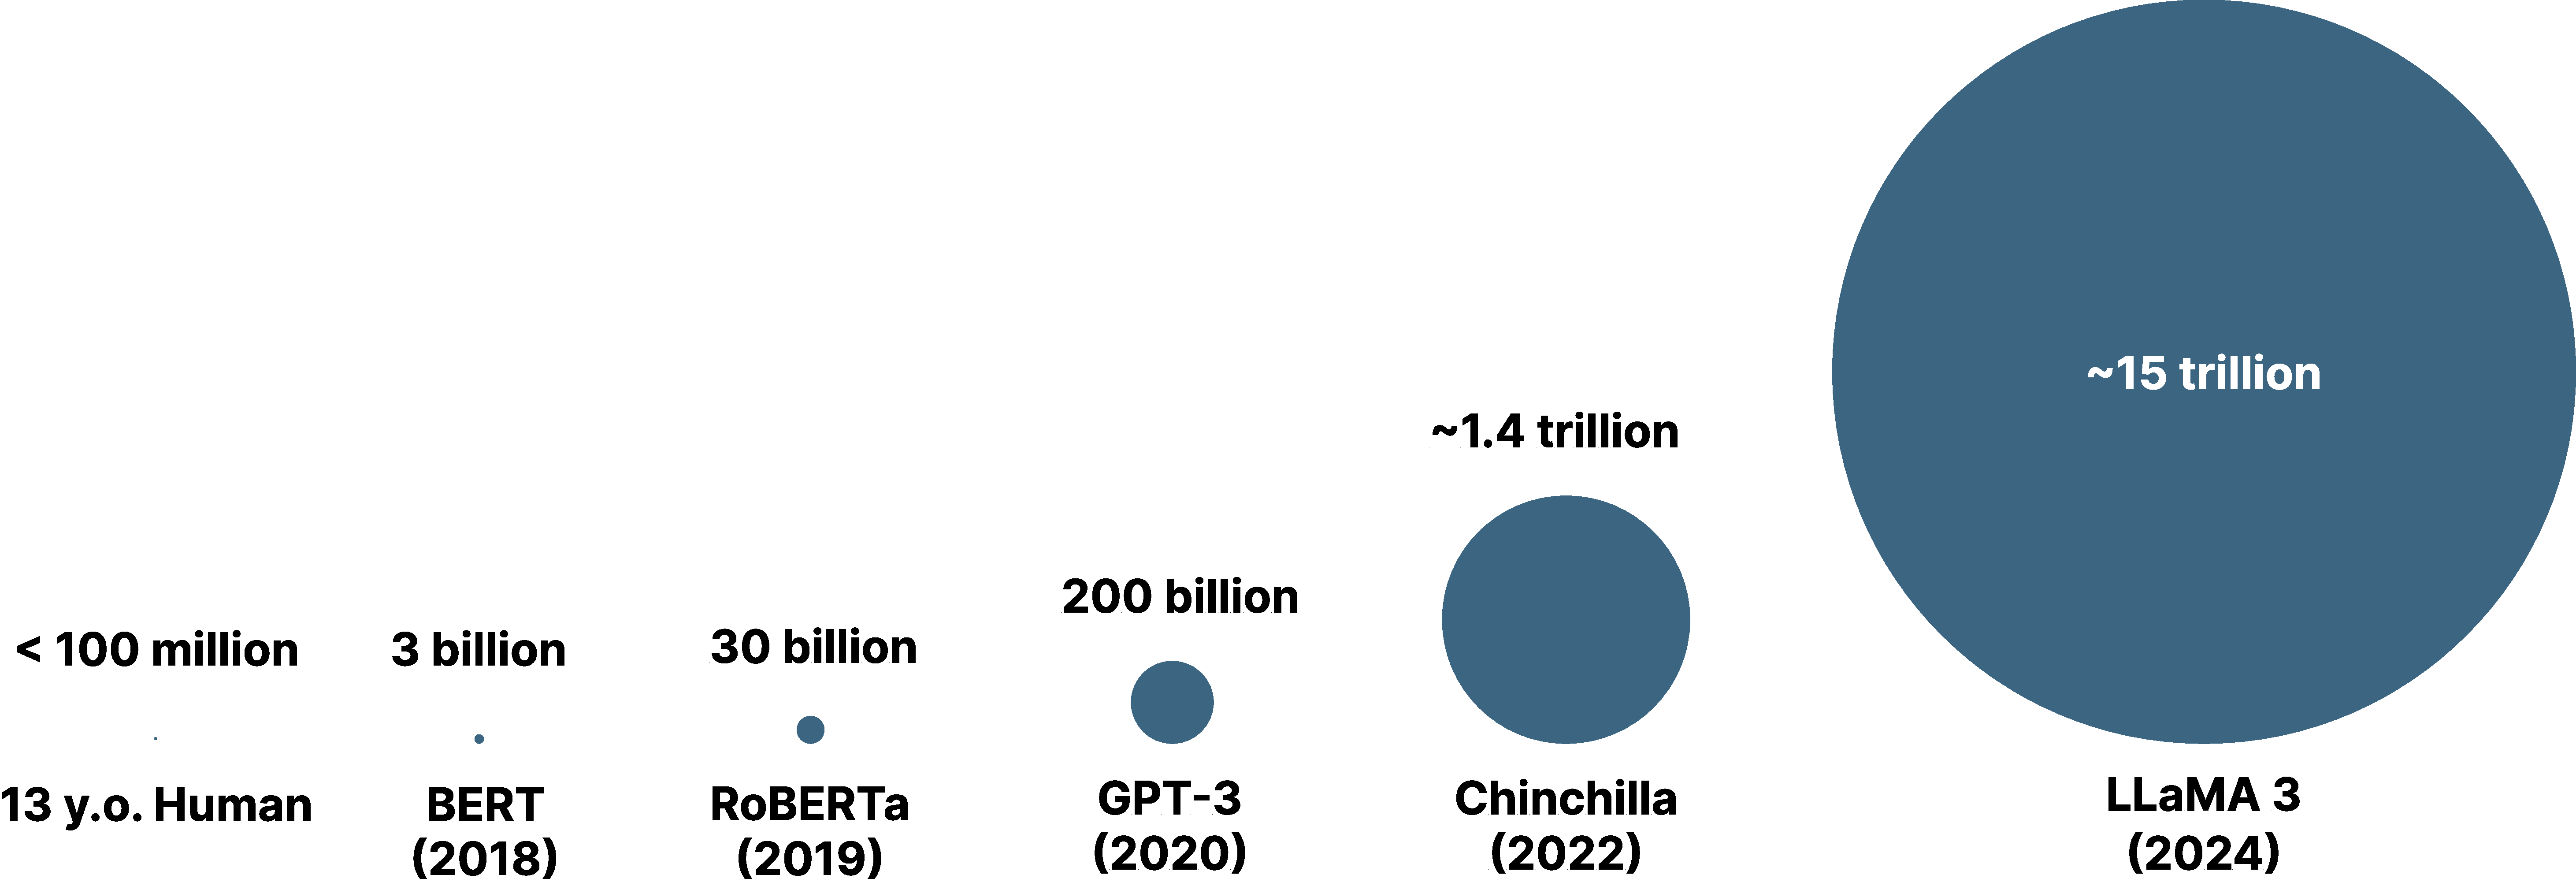
\includegraphics[width=0.7\textwidth]{chapters/background/figures/data_comparison.pdf}
    \caption{Comparison of data scales used by different language modeling approaches. Humans are estimated to observe less than 100 million words by the age of 13.}
    \label{fig:data-comparison}
\end{figure}

% If children acquire sophisticated language capabilities from only a few million words per year, what can this teach us about building more efficient and interpretable language models?

While current research directions for improving small model efficiency largely center on optimization and architectural innovations, these efforts are generally exploratory; they lack an underlying thesis for how to train models more efficiently. To make more grounded and robust progress in developing efficient training paradigms, it is valuable to establish a guiding framework or set of principles. One promising approach is to draw inspiration from how humans learn. The brain is a biologically constrained system that achieves remarkable linguistic competence with limited resources. \cref{fig:data-comparison} visualizes the order of magnitude difference that language models are trained on versus the amount of data humans perceive. By studying cognitive processes and human language acquistion, we argue that we can derive strategies that may inform more efficient model training.

One particularly relevant insight is the Goldilocks principle \citep{kidd2012goldilocks}, which shows that infants prefer stimuli that are neither too simple nor too complex. This suggests that humans learn language optimally when input difficulty is finely calibrated. Children also benefit from rich, contextualized input \citep{bergelson2015early, weizman2001lexical}, where language is embedded in meaningful interaction. Cognitive models of predictive processing~\citep{caucheteux2023evidence} indicate that human learners excel in environments that balance familiar patterns with novel stimuli. 

These findings collectively support the idea that language models could benefit from carefully structuring the order in which inputs are shown to the model. This idea has motivated a growing interest in cognitively grounded data augmentation and curriculum design strategies for training small language models.

\subsection{Curriculum Learning}

\thesishl{Curriculum learning} draws inspiration from how children acquire language progressively rather than all at once. As \citet{bengio2009curriculum} formalized, this approach involves structuring training to begin with easier inputs and gradually increase complexity over time, rather than exposing models to randomly shuffled data of uniform difficulty. Complexity in the training of a language model can arise across several dimensions:

%This paradigm also maps naturally onto human language production: children do not produce all linguistic phenomena simultaneously, but instead progress from babbling to simple utterances, and eventually to complex syntax and abstract meaning. The BabyLM Challenge \citep{warstadt2023babylm1} provides an ideal testbed for exploring these ideas under cognitively plausible constraints.

% A key challenge in curriculum learning is how to define what makes a training example “easy” or “hard” for a given language model? Learning difficulty can arise from multiple facets of the training setup. For instance, difficulty can be defined via linguistic features of the training data (e.g. sentence length, syntactic complexity, or vocabulary frequency), via model-based metrics (such as computing perplexity or an auxiliary model's loss on a given set of data), or even via human-annotated scores (for example, readability or “surprisal”) \citep{soviany2022curriculum}. Moreover, curriculum learning can be applied to aspects of the training pipeline other than the data. These include:   %In practice, researchers often combine these signals (or use a dynamic curriculum that re-evaluates difficulty periodically) to keep training material in the “zone of proximal development” (or “Goldilocks” zone); that is, neither too easy (so that the model is not challenged) nor too hard (so that learning is not stalled). Current research has explored several dimensions of curriculum learning in NLP.

\paragraph{Dynamic data sampling} The most common variant of curriculum learning defines training complexity as the `difficulty' of the training examples shown to a model. A key challenge in this framing is how to define what makes a training example “easy” or “hard” for a given language model?  For instance, difficulty can be defined via linguistic features of the training data (e.g. sentence length, syntactic complexity, or vocabulary frequency) \citet{campos2021curriculum, kocmi2017curriculum, liu2018curriculum}, via model-based metrics (such as computing perplexity or an auxiliary model's loss on a given set of data) \citet{sachan2016easy, lalor2020dynamic}, or even via human-annotated scores (for example, readability or “surprisal”) \citep{soviany2022curriculum}. 

\paragraph{Progressive vocabulary exposure} A secondary axis to apply curriculum learning to is the vocabulary of a language model. Studies show children begin with a limited lexicon that expands gradually (by 8-10 words per day) \citep{fenson1994variability, bergelson2015early, weizman2001lexical}, focusing first on concrete nouns and verbs. In contrast, language models traditionally start with a complete vocabulary. Recent work has begun exploring frequency-based vocabulary scaffolding \citep{soviany2022curriculum} so that models gradually acquire a larger vocabulary, akin to human language learners. 

\paragraph{Graduated learning objectives} Curriculum learning can also be applied at the level of the objective function used to train a language model. Standard language modeling objectives (such as MLM) that require identifying a masked token as one of possibly thousands of vocabulary items can be quite challenging from the outset. Some approaches have explored beginning with simpler prediction tasks (e.g. part-of-speech classification) before tackling more complex ones, similar to how children grasp broad categories before mastering precise lexical distinctions \citep{markman1990constraints}. For instance, \citet{bai2022better} (mapping rare words to hypernyms) and \citet{wang2023language, cui2022lert} (using auxiliary tasks such as POS tagging) illustrate how objective curricula can smooth the learning signal. These ideas are also inspired by psycholinguistic theories (e.g. \citet{alishahi2010computational, gleitman1990structural}) that children first learn coarse linguistic categories and later generalize to a full lexicon.

\vspace{1em}

While these ideas have been explored individually, there remains significant opportunity for developing more integrated approaches. There is currently no unified framework that systematically implements and evaluates these strategies, especially in small-scale language modeling. Such a framework would be particularly valuable for understanding how different curriculum dimensions (i.e. vocabulary progression, data ordering, and learning objectives) interact and complement each other when training small language models. By developing methods to compare and combine these approaches, we could gain deeper insights into which aspects of human-like learning are most beneficial for model efficiency and generalization.

\subsection{Syntactic Generalization}

While curriculum learning provides a framework for structuring the learning process, another key challenge in language modeling is ensuring robust generalization to novel linguistic structures. This challenge mirrors a fundamental aspect of human language acquisition: the ability to understand and produce grammatical constructions that may not have been explicitly observed during learning. From an early age, children demonstrate an impressive capacity to abstract syntactic patterns and apply them productively, even with limited exposure \citep{yang2013poverty, legate2002empirical}. This capacity suggests that humans possess strong inductive biases that enable generalization from sparse and noisy input.

As an illustrative example, take the sentence, ``After lunch, the kids zambled through the garden, giggling and chasing butterflies.'' Even though `zambled' is a made-up word, we can nonetheless infer its syntactic category (verb), morphological structure (past participle), and approximate meaning based on surrounding cues (e.g. `to run joyfully'): a phenomenon known as ``syntactic bootstrapping" \citep{gleitman1990structural, naigles1990children}. This ability highlights the importance of syntax as a scaffold for lexical learning and supports the hypothesis that grammatical structures provide a backbone for interpreting linguistic input. By contrast, language models struggle to incorporate syntactic cues in a similar way to humans due to two key properties inherent to language modeling:

\paragraph{Frequency Bias} While human learners generalize from structure, language models internalize surface-level frequency statistics due to their maximum likelihood training objectives. This results in a strong bias toward frequent tokens and can obscure the model's true syntactic capabilities \citep{feldman2020does, haviv2023understanding}. Human learners, by comparison, rely on structural cues rather than frequency alone, allowing them to recognize grammatical roles even for novel or rare words \citep{tomasello2003constructing, clark2020emergence}.

\paragraph{Representation Degeneration} Frequency-driven learning can also lead to representation collapse, where embeddings for rare tokens are poorly differentiated. This degeneration leads to \thesishl{anisotropy} in the representation space of embeddings; a phenomenon where the embeddings of all infrequent words converge into a narrow subspace \citep{ethayarajh2019contextual}. In contrast, human mental lexicons maintain separable, richly structured representations for even infrequent words \citep{murphy2002bigbook}.

% \paragraph{Scaling Limitations} Larger model sizes are often needed to approximate the statistical properties of infrequent words, posing a challenge for efficiency and interpretability. Human learners, however, achieve high generalization with dramatically fewer parameters—suggesting the potential of syntactic cues as a source of inductive bias that supports efficient learning from small data \citep{tomasello2003constructing, clark2020emergence}.

% To address these challenges, recent approaches have drawn inspiration from how children integrate linguistic structure into word learning:

% \paragraph{Linguistic Feature Integration} Echoing how children rely on morphosyntactic cues to infer category and meaning \citep{gleitman1990structural, naigles1990children}, several methods enhance token representations with morphological, syntactic, or lexical-semantic information \citep{salle2018incorporating, vulic2017morphfitting, cui2022lert, diehlmartinez2023climb}. These augmentations allow models to generalize more effectively, especially for underrepresented vocabulary.

% \paragraph{Representation Space Optimization} Techniques that mitigate anisotropy in embedding spaces aim to recover a more human-like separation of meanings. By filtering out dimensions dominated by frequency or noise, these methods promote models to learn syntactic organization \citep{arora2016simple, mu2018all, bis2021too}.

% \paragraph{Objective Calibration} Alternative training objectives and regularization strategies seek to reduce frequency bias by explicitly rewarding syntactic consistency and discouraging overfitting to frequent items \citep{gong2018frage, gao2018representation}. These interventions embed a structural bias into learning, allowing even small models to better generalize from limited input—mirroring the efficiency of human learners.

\vspace{1em}

 Advancing syntactic generalization in models, especially those constrained in size or training data, requires more principled integration of linguistic theory and cognitive insight.

\subsection*{From Cognitive Theory to Computational Practice}

Integrating principles from human learning into language modeling marks a significant shift in how we think about model development. Rather than focusing solely on architectural innovations or computational efficiency, we emphasize drawing from cognitive and developmental theories to design learning protocols that mirror human acquisition. By aligning our training approaches with human learning principles, we may uncover not only more efficient models, but also models that offer deeper interpretability and insight into the nature of language learning itself.

This thesis explores two complementary approaches to human-inspired language modeling. First, in Chapter 3, we introduce Curriculum Learning for Infant-inspired Model Building (CLIMB), a framework developed for the BabyLM Challenge. CLIMB explores three cognitively inspired curriculum learning strategies: vocabulary progression, data difficulty ordering, and graduated learning objectives. Through this work, we aim to evaluate the effectiveness of curriculum learning under real-world data constraints, testing whether models can learn language more like humans do by following a developmentally plausible learning trajectory.

Building on these insights about structured learning, Chapter 4 addresses a fundamental challenge in language modeling: how to achieve robust syntactic generalization without relying on increasingly large models. We present \texttt{Syntactic Smoothing}, a method inspired by how children leverage syntactic knowledge to understand novel vocabulary items. This approach distributes learning signals across syntactically similar tokens, helping models better represent infrequent words while maintaining strong language modeling capabilities.

Together, these chapters demonstrate how insights from human language acquisition can inform more efficient approaches to language modeling, from the macro-level structure of learning (curriculum design) to the micro-level mechanics of representation (syntactic generalization).